\begin{figure}[htbp]

\begin{center}
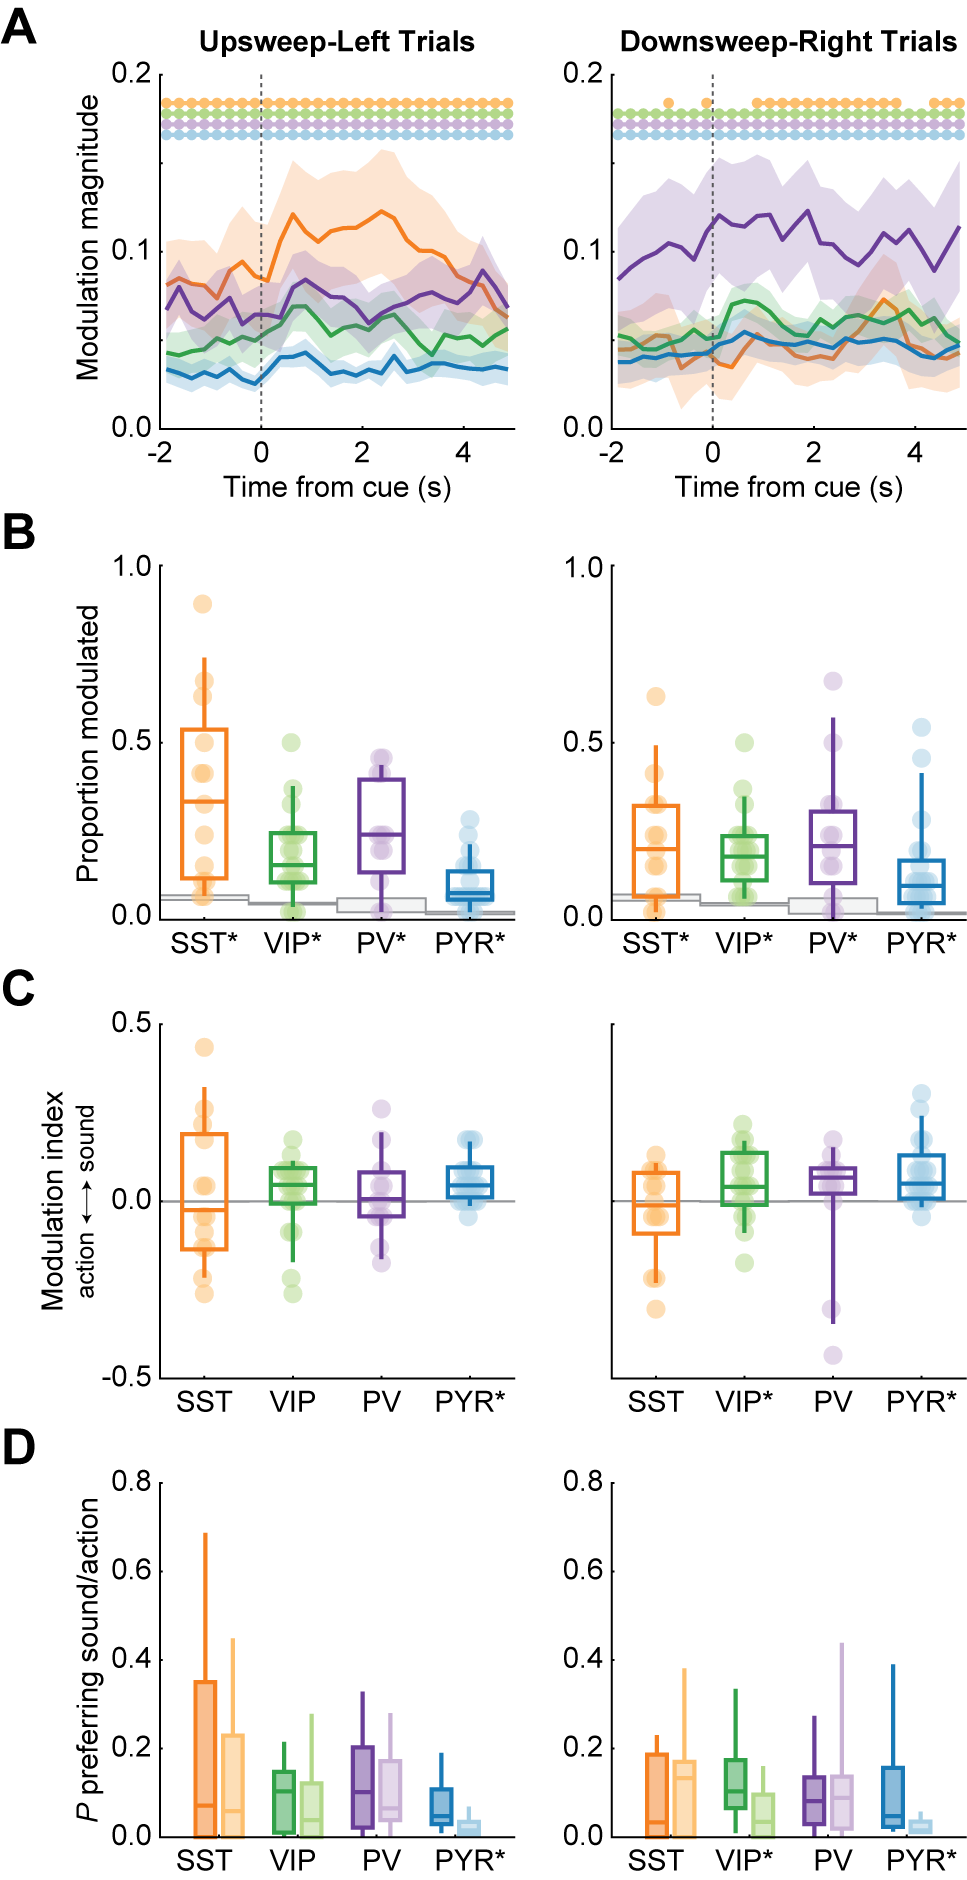
\includegraphics[width=8.7cm]{Figures/Chapter4/Fig8} 
\end{center}

\caption[Context-related modulation]
{Context-related modulation. Modulation by the current rule was examined under matched trial conditions: upsweep trials in which a left choice was rewarded (left), and downsweep trials in which a right choice was rewarded (right). (A) Modulation magnitude $M_{\mathit{rule}}(t)$ with respect to the rule governing the current trial (sound vs. action), plotted as in Figure \ref{fig:Fig6}A. Solid circles indicate time bins where $M_{\mathit{rule}}(t)$ differed significantly from chance ($p<0.05$, Wilcoxon signed-rank test vs. shuffle) within SST (orange), VIP (green), PV (purple), and PYR populations (blue). (B) The proportion of each cell population, $P_{\mathit{rule}}$, that exhibited significant modulation associated with the current rule. (C) The mean modulation index $\bar{I}_{\mathit{rule}}$, calculated from the first 5 s of the trial. (D) The proportion of each cell population exhibiting a significant preference for the sound ($P^+$; dark shading) and action rule ($P^-$; light shading), represented respectively in paired box plots. Asterisks in B--C indicate significant differences from the null distribution for each cell type; in D, they indicate significant differences between $P^+$ and $P^-$ within each cell type; both were assessed at $\alpha = 0.05$, Wilcoxon signed-rank test. $N=$ 13 SST, 19 VIP, 12 PV, and 20 PYR populations. All plots presented as in Figures \ref{fig:Fig6}--\ref{fig:Fig7}}

\label{fig:Fig8}
\end{figure}

% {Context-related modulation. Modulation by the current rule was examined under matched trial conditions: upsweep trials in which a left choice was rewarded (left), and downsweep trials in which a right choice was rewarded (right). (A) Modulation magnitude $M_{\mathit{rule}}(t)$ with respect to the rule governing the current trial (sound vs. action), plotted as a function of time relative to the sound cue.  Solid lines, mean; shading, SEM. Solid circles above indicate time bins where $M_{\mathit{rule}}(t)$ differed significantly from chance ($p<0.05$, Wilcoxon signed-rank test). (B) The proportion of each cell population, $P_{\mathit{rule}}$, that exhibited significant modulation associated with the current rule. (C) The mean modulation index $\bar{I}_{\mathit{rule}}$, calculated from the first 5 s of the trial. (D) The proportion of each cell population exhibiting a significant preference for the sound ($P^+$; dark shading) and action rule ($P^-$; light shading), represented respectively in paired box plots. Asterisks in B--C indicate significant differences from the null distribution for each cell type; in D, they indicate significant differences between $P^+$ and $P^-$ within each cell type; both were assessed at $\alpha = 0.05$, Wilcoxon signed-rank test. All plots presented as in Figures \ref{fig:Fig5}--\ref{fig:Fig6}}